\chapter{Introduction}
\label{intro}
Universities, science centers and other institutions has the need for equipment that demonstrates physical phenomena in interesting and audience friendly ways. An example of this is a Double Resonant Solid State Tesla Coil (DRSSTC). This is a contraption that by the use of high voltage generates a sequence of electrical discharges. When these discharges happen in air a sound wave is generated. By modulating the frequencies of these discharges one can generate sound with different tones. A DRSSTC can in this way be made into a musical instrument.
There is no big commercial or academic community for tesla coils, but tesla coils are mostly designed and used as a hobby. There are a few people sharing their designs on the internet that most of the tesla coil designs are based on. Few or none of these substantiate design choices or assumptions with physics and math. This thesis will attempt to substantiate the design choices done in the driver for a musical dual resonant solid state tesla coil.

\Cref{fig:teslabano} shows a DRSSTC in use where a streamer has formed from the top load to a grounded copper object.

\begin{figure}[ht]
    \centering
    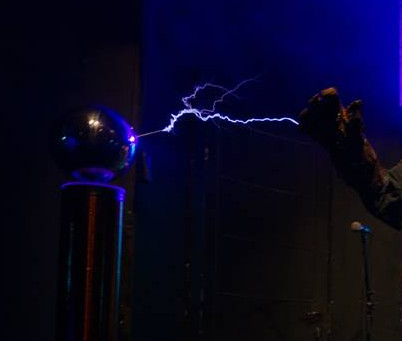
\includegraphics[width=0.6\textwidth]{img/teslabano.jpg}
    \caption{A tesla coil in use}
    Photo: Sindre Vaskinn Hunn
    \label{fig:teslabano}
\end{figure}

\section{Tesla Coil}
\label{tesla}
%http://www.tfcbooks.com/tesla/contents.htm
The Tesla Coil is a form of resonant transformer invented by Nikolai Tesla and used for experiments with artificial illumination \citep{5570149}. A resonant transformer consists of two inductively coupled coils, each loaded with a capacitance such that they get the same resonance frequencies. The resonant transformer has since gotten a lot of applications, among others; RFID, NFC, and Wireless charging. The resonant transformer in the form of the Tesla Coil has also become a popular entertainment device.
%Death ray
%Entertainment

\section{Earlier work}
%Who has done work on this before? steve4hv, pupman, scantesla, loneoceans.
Some of the people who have done work on DRSSTC in the hobbby community are; Steve Ward \Citep{stevehv}, Jimmy Hynes \Citep{chunkyboy86}, Terry Fritz \Citep{terrel}, Steve Conner \Citep{conner}, Dan McCauley \Citep{easternvoltage}, and the tesla coil mailing list \Citep{pupman}. Among these there are few disagreements on how a tesla coil should be designed, there are few variations on the resonant circuit, but slightly more variation on the low voltage controlling side. Some use a preset oscillator to drive the resonant circuit, while others use feedback from either the primary or secondary resonant circuits.

There has been developed an drsstc tesla coil driver by Steve Ward witch other people have designed variations on \Citep{ud27}.

Simulation software for the resonant circuitry of tesla coils called Scantesla have been written \Citep{scantesla}.

Guidelines for the design of the resonant circuits can be found at most of the above mentioned sites.

A modular back plane based tesla coil driver implementation have been designed and implemented by the author together with other members of Omega Verksted\footnote{Omega Verksted is a association of electronics and hobby interested students at the Norwegian University of Science and Technology (NTNU) founded in 1971.}. This is based on earlier designs by members of Omega Verksted, the last major implementation at Omega Verksted was done in 2009 mostly by Dewald de Bruyn.

%Onetesla sells commercially

%Tables for coil aspect ratios.
